% IEEE journal template, with the 10pt two-column format required by TWC.
% Compile from paper/; keep the IEEEtran fonts and page dimensions.
% Select T1 before the class selects Times, including under XeTeX/Tectonic.
\RequirePackage[T1]{fontenc}
\documentclass[10pt,journal,letterpaper]{IEEEtran}
\usepackage{amsmath,amssymb,bm,booktabs,array}
\usepackage{graphicx}
\usepackage{cite}
\usepackage{enumitem}
\usepackage{algpseudocode}
\usepackage[hidelinks]{hyperref}
\graphicspath{{figures/}}
\interdisplaylinepenalty=2500

\newcounter{algorithm}
\renewcommand{\thealgorithm}{\arabic{algorithm}}
\algrenewcommand\algorithmicrequire{\textbf{Input:}}
\algrenewcommand\algorithmicensure{\textbf{Output:}}

\newcommand{\CN}{\mathcal{CN}}
\newcommand{\E}{\mathbb{E}}
\newcommand{\I}{\mathbf{I}}
\newcommand{\vect}{\operatorname{vec}}
\newcommand{\tr}{\operatorname{tr}}
\newcommand{\diag}{\operatorname{diag}}
\newcommand{\logit}{\operatorname{logit}}
\newcommand{\sigmoid}{\operatorname{sigmoid}}
\newcommand{\clip}{\operatorname{clip}}
\newcommand{\relu}{\operatorname{Re}}
\newcommand{\imag}{\operatorname{Im}}
\newcommand{\norm}[1]{\left\lVert#1\right\rVert}

\title{Generative-Model-Aided Grant-Free Random Access for GNSS-Independent MIMO-AFDM Satellite IoT Systems}
% Author order and IEEE membership grades supplied by the author.
\author{Bo~Wang,~\IEEEmembership{Student~Member,~IEEE,}
Wenpeng~Jing,~\IEEEmembership{Member,~IEEE,}
Zhiqun~Hu,~\IEEEmembership{Member,~IEEE,}
Shirui~Zuo,~\IEEEmembership{Student~Member,~IEEE,}
and~Changhao~Liu,~\IEEEmembership{Student~Member,~IEEE}%
\thanks{All authors are with Beijing University of Posts and
Telecommunications (e-mails: wangb@bupt.edu.cn;
[Wenpeng Jing: e-mail to be added]; [Zhiqun Hu: e-mail to be added];
[Shirui Zuo: e-mail to be added]; [Changhao Liu: e-mail to be added]).}}

\begin{document}
\bstctlcite{IEEEcontrol}
\maketitle
\begin{abstract}
This paper investigates grant-free random access in low Earth orbit
satellite Internet-of-Things systems without global navigation satellite
system (GNSS) assistance, where devices operate without time and frequency
precompensation. We propose a multi-frame affine frequency division
multiplexing (AFDM) transmission scheme that accommodates large differential
delays and Doppler shifts across devices and analyze its input-output
relationship. Based on this model, we learn a score-based generative channel
prior directly from AFDM
effective-channel samples, without imposing sparse or grid-aligned channel
assumptions. From the learned prior, we construct a minimum mean-squared
error (MMSE) channel denoiser that also quantifies estimation uncertainty.
We then incorporate the denoiser into a message-passing
(MP) receiver with two modules: multi-frame linear estimation (MFLE), which
suppresses inter-user interference; and generative-prior-aided joint
denoising (GPJD), which jointly updates channel and activity estimates. GPJD
employs a density-ratio estimator that learns the likelihood ratio required
for activity detection. The two modules
iteratively exchange soft information for joint activity detection and
channel estimation (JADCE). Numerical simulations demonstrate that the
proposed receiver outperforms the baseline receiver in activity detection
and channel estimation, while requiring fewer pilot frames to reach the same
channel-estimation target.
\end{abstract}
\begin{IEEEkeywords}
Affine frequency division multiplexing, grant-free
random access, joint activity detection and channel estimation,
score-based generative models.
\end{IEEEkeywords}

\section{Introduction}
\label{sec:introduction}

Sixth-generation (6G) wireless networks are expected to provide ubiquitous
connectivity for a massive number of Internet-of-Things (IoT) devices
\cite{cai2026,xu2026}. To serve devices in remote areas with limited terrestrial
coverage, low Earth orbit (LEO) satellites complement cellular networks for
applications such as smart agriculture and climate monitoring \cite{shen2025,kodheli2021}. These
power-limited devices transmit short packets sporadically, with only a small
fraction active at a given time \cite{shen2025,cai2026,mei2022}. In grant-based random
access, handshaking before transmission incurs significant
signaling overhead, while the long propagation delay of terrestrial-satellite links
further increases access latency \cite{cai2026,xu2026}. Accordingly, grant-free
random access (GFRA) allows active devices to transmit pilots and data directly
without first obtaining a grant \cite{cai2026,xu2026}.

Supporting GFRA over LEO links requires handling large delays and Doppler shifts
caused by long propagation distances and high satellite mobility. The 3rd Generation
Partnership Project (3GPP) Release 17 framework addresses these effects through
device-side precompensation assisted by the global navigation satellite system
(GNSS) \cite{3gpp38300}. With such precompensation, many existing satellite GFRA
schemes assume perfect compensation or small residual delays and Doppler shifts at
the receiver \cite{shen2025}. Frequent estimation and compensation increase
energy consumption and reduce battery lifetime, making these schemes less suitable
for power-limited remote IoT devices \cite{shen2025}. This motivates reducing
dependence on GNSS, consistent with the GNSS-independent operation considered in the
Release 19 study on satellite access \cite{3gpp22865}. With reduced reliance on
device-side precompensation, the satellite receiver must accommodate
large differential delays and Doppler shifts, which can cause severe inter-symbol
and inter-carrier interference in conventional orthogonal frequency division
multiplexing (OFDM) systems \cite{shen2025,huang2026}.

Orthogonal time frequency space (OTFS) modulation exploits the quasi-static
properties of channels in the delay--Doppler domain to mitigate these effects
\cite{shen2025,hadani2017}. In \cite{shen2025}, multi-frame OTFS transmission
handles large differential delays and Doppler shifts at the satellite receiver,
allowing devices to operate without GNSS assistance or precompensation of these
offsets. Affine frequency division multiplexing (AFDM)
offers a low-complexity modulation structure based on one-dimensional chirp
signals \cite{ding2026,huang2026}. Its modulator can be implemented using a
single inverse fast Fourier transform and two stages of pointwise chirp
multiplication \cite{bemani2022}.

Since device activity and channels are unknown at the receiver, AFDM-GFRA
requires joint activity detection and channel estimation (JADCE)
\cite{ding2026}. Existing
methods exploit sporadic device activity to formulate JADCE as a compressed sensing
(CS) problem and incorporate structured priors to model channel sparsity
\cite{shen2025,ding2026,ke2020}. The scheme in \cite{ding2026} further uses a graph neural
network to adaptively learn sparsity patterns, while retaining a predefined
delay--Doppler grid for the sparse channel representation. In practical
propagation environments, significant power leakage caused by fractional Doppler
shifts and fractional time delays can weaken the sparsity of the effective channel
matrix \cite{huang2026}. This motivates learning effective-channel
priors from data to capture channel structures beyond the assumed sparse
representation \cite{cai2026,huang2026}.

Score-based generative models learn channel priors from samples by estimating the
score function of the channel distribution \cite{song2019,arvinte2023}. In
\cite{huang2026}, score-based learning is performed directly on the AFDM effective
channel to address fractional delay--Doppler off-grid leakage in channel estimation.
For massive random access, \cite{ying2026} proposes a two-stage algorithm that first
identifies active devices through a Transformer-based detector and then uses
generative diffusion models for joint channel estimation and data detection.
However, both approaches rely on iterative posterior sampling, which requires
repeated score function evaluations and incurs substantial computational cost
\cite{huang2026,ying2026}.

The score-based turbo message passing (STMP) algorithm in \cite{cai2026}
incorporates generative channel priors for JADCE without iterative posterior
sampling. Through Tweedie's formulas, first- and second-order score networks provide
channel estimates and variances for single-step minimum mean-squared error (MMSE)
denoising under equivalent additive white Gaussian noise (AWGN) observations.
For activity detection, STMP computes activity probabilities using Gaussian extrinsic messages
obtained by projecting the channel posterior onto a Gaussian distribution
\cite{cai2026}. For a non-Gaussian channel prior, however, matching the mean and
variance does not generally preserve the marginal likelihood. The relation between
density ratios and class probabilities \cite{menon2016} offers an alternative:
estimating the activity likelihood ratio directly from samples, without relying
on this Gaussian approximation or explicitly evaluating the marginal likelihood.

Against this background, we investigate GNSS-independent AFDM-GFRA for
LEO satellite IoT systems. Our main contributions are summarized as follows:

\begin{enumerate}[label=\arabic*)]
\item We propose a multi-frame AFDM transmission scheme that accommodates large
differential delays and Doppler shifts at the satellite receiver without
requiring device-side precompensation. We derive the input-output relationship
and show that the effective channels across frames differ only by
Doppler-induced phase rotations.
Additional pilot frames therefore provide more observations without
increasing the number of channel coefficients to be estimated. Compared with
the multi-frame OTFS representation of Shen et al.~\cite{shen2025}, the
effective channel matrix in our model contains fewer coefficients.

\item We learn a score-based generative prior for AFDM effective channels without
imposing sparse or grid-aligned channel assumptions. Building on Tweedie's
formula and the relation between denoiser derivatives and estimation
uncertainty, we develop a channel denoiser that provides both channel estimates
and average variance without requiring a separately trained variance model.

\item We develop a message-passing JADCE receiver whose generative-prior-aided
joint denoising (GPJD) module combines the proposed channel denoiser with a
learned density-ratio estimator. The estimator enables activity detection
under the learned channel prior without explicit marginal-likelihood
evaluation. GPJD iteratively exchanges extrinsic messages with the
multi-frame linear estimation (MFLE) module, which jointly processes the
pilot frames to suppress inter-user interference. Simulations show that
the proposed receiver outperforms the STMP baseline adapted to AFDM in activity
detection and channel estimation, and requires fewer pilot frames to achieve
the same channel-estimation accuracy.
\end{enumerate}

The remainder of this paper is organized as follows. Section~\ref{sec:system}
presents the system model and the multi-frame AFDM input--output relationship.
Sections~\ref{sec:algorithm}--\ref{sec:overall} describe the message-passing
framework, the learned channel denoiser and activity classifier, and the overall algorithm with its computational
complexity analysis, respectively. Section~\ref{sec:simulations} presents the
simulation results. Section~\ref{sec:conclusion} concludes this paper.


\noindent\textit{Notation:} Bold lowercase and uppercase letters denote vectors and matrices, respectively. $\CN(\bm\mu,\bm\Sigma)$ denotes a proper complex Gaussian distribution \cite{neeser1993}.
$\|\cdot\|_F$ denotes the Frobenius norm;
$(\cdot)^{\mathsf H}$ and $\tr(\cdot)$ denote conjugate transpose and trace.
$\vect(\cdot)$ stacks matrix columns, and $\I_n$ is the $n\times n$ identity matrix.

\section{System Model}
\label{sec:system}

We consider a LEO satellite-enabled grant-free random access system
as illustrated in Fig.~\ref{fig:system-multiframe}, where AFDM is adopted
to mitigate the doubly dispersive effect \cite{huang2026} inherent in
terrestrial-satellite links (TSLs). The system comprises $K$
single-antenna terrestrial devices that communicate with a LEO satellite
equipped with a uniform planar array (UPA) consisting of $M=M_yM_z$
antennas. During each transmission block, active devices share the same
time-frequency resources to transmit their pilots to the satellite.
Additionally, we assume that these terrestrial devices operate without
GNSS assistance and do not pre-compensate for delay and Doppler shifts
\cite{shen2025}.

\begin{figure}[!t]
\centering
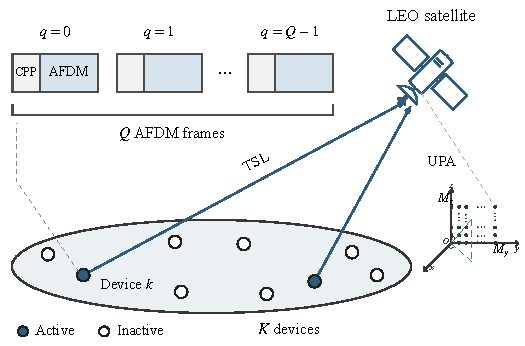
\includegraphics[width=\linewidth]{system_multiframe.pdf}
\caption{LEO satellite grant-free access with multi-frame AFDM pilot
transmission. The insets show the frame structure of active device $k$
and the satellite UPA. Device activity is fixed over the $Q$ frames.
Satellite, footprint, and array artwork
is adapted from \cite{shen2025}.}
\label{fig:system-multiframe}
\end{figure}

\subsection{Terrestrial-Satellite Link Model}

The TSLs experience fast variations due to the high mobility of the LEO
satellite. Hence, this time variation and multipath propagation require a
doubly dispersive channel model for accurate TSL characterization
\cite{shen2025}. For stationary terrestrial devices, the Doppler shift
$\nu_k$ is assumed to be common to all propagation paths within the same
TSL, since the long satellite-to-ground distance leads to only a small
angular spread across multipath components \cite{huang2026}.
The angles of arrival of these paths are approximately identical,
so that they
share the same array response vector $\mathbf a_k$ \cite{li2023}.
We assume that the channel in the delay-Doppler domain remains
approximately constant over the $Q$ frames of a transmission block
\cite{shen2025}. Then, taking the start of the block as $t_{\rm c}=0$,
the channel impulse response from the $k$th device to the satellite
after common-delay compensation by $\tau_{\rm c}$ can be represented as

\begin{equation}
 \mathbf h_k(t_{\rm c},\tau)
 =\mathbf a_k\sum_{\ell=1}^{L_k}g_{k\ell}
 e^{\mathrm j2\pi\nu_k t_{\rm c}}\delta(\tau-\tau_{k\ell}),
 \label{eq:physical-channel}
\end{equation}
where $k=1,\ldots,K$, and $L_k$ is the number of physical paths.
Here, $\tau_{k\ell}=\widetilde\tau_{k\ell}-\tau_{\rm c}$ represents the
differential delay for the $\ell$th path from the $k$th device to the
satellite, where $\widetilde\tau_{k\ell}$ and $\tau_{\rm c}$ denote the
propagation delay and common delay, respectively.
The common delay corresponds to the propagation time between the satellite
and the closest point on Earth within the beam footprint. Additionally,
$g_{k\ell}$ is the path gain of the $\ell$th path, $\delta(\cdot)$ is the
Dirac delta function, and $\mathrm j^2=-1$.

Then, the array response vector $\mathbf a_k$ can be expressed as
\begin{equation}
 [\mathbf a_k]_{n_z+M_zn_y}
 =e^{\mathrm j2\pi(d_yn_y\mu_{y,k}+d_zn_z\mu_{z,k})/\lambda},
 \label{eq:upa}
\end{equation}
where $n_z=0,\ldots,M_z-1$, $n_y=0,\ldots,M_y-1$,
$\lambda$ is the wavelength, and $d_y$ and $d_z$ are the spacings between
adjacent antennas along the $y$- and $z$-axes, respectively. The
directional cosines along these two axes are denoted by $\mu_{y,k}$ and
$\mu_{z,k}$, respectively.

\subsection{Transmission Scheme}
\label{sec:transmission-scheme}

The multi-frame AFDM transmission scheme is proposed to handle the large
differential delay and Doppler shift. In this scheme, each active device
transmits pilots over $Q$ consecutive frames within one transmission
block. While AFDM modulation and demodulation are performed separately
for each frame, the receiver jointly processes the resulting observations.
Specifically, in the $q$th AFDM frame, $q=0,\ldots,Q-1$, the $k$th
device transmits the known pilot vector $\mathbf p_{qk}\in\mathbb C^N$,
where $N$ is the number of chirp subcarriers shared by the devices.

We construct the pilot matrices as
$\mathbf P_k=[\mathbf p_{0k},\ldots,\mathbf p_{Q-1,k}]^{\mathsf T}$
and $\mathbf P=[\mathbf P_1,\ldots,\mathbf P_K]\in\mathbb C^{Q\times KN}$,
where $(\cdot)^{\mathsf T}$ denotes transpose.
We impose the condition that
$\mathbf P\mathbf P^{\mathsf H}=KE_p\I_Q$, where
$\|\mathbf p_{qk}\|^2=E_p$ for all $k$ and $q$
\cite{cai2026}.

Through the inverse discrete affine Fourier transform (IDAFT)
\cite{ding2026}, $\mathbf p_{qk}$ is mapped to the time-domain signal
given by

\begin{equation}
 s_{qk}[t]=\frac{1}{\sqrt N}\sum_{n=0}^{N-1}
 [\mathbf p_{qk}]_ne^{\mathrm j2\pi(c_1t^2+c_2n^2+nt/N)},
 \label{eq:afdm-time-signal}
\end{equation}
where $t=0,\ldots,N-1$, and $c_1$ and $c_2$ are AFDM modulation
parameters.
The corresponding discrete affine Fourier transform (DAFT) matrix is
\begin{equation}
 \begin{gathered}
 \mathbf F_{\rm A}
 =\left[\frac{1}{\sqrt N}e^{-\mathrm j2\pi(c_2r^2+rt/N+c_1t^2)}
 \right]_{r,t=0}^{N-1}
 \end{gathered}.
 \label{eq:daft}
\end{equation}

Assume that the chirp-periodic prefix (CPP) duration is greater than
or equal to the maximum differential delay, i.e.,
$N_{\rm CPP}T_s\geq\max_{k,\ell}\tau_{k\ell}$.
Here $T_s=1/(N\Delta f)$ is the sampling interval, with $\Delta f$
denoting the subcarrier spacing, and
$T_{\rm frame}=(N+N_{\rm CPP})T_s$ is the duration of an AFDM frame
with CPP.

Next, we use a continuous-time AFDM waveform
\cite{bemani2023thesis} with a chirp-periodic prefix extension
\cite{bemani2022} to model fractional delays. The basis function for
chirp subcarrier $n$ at time $\xi T_s$ is given by
\begin{equation}
 \varphi_n(\xi)=\frac{1}{\sqrt N}
 e^{\mathrm j2\pi[c_2n^2+c_1\xi^2+nw_\xi/N-\zeta_n(w_\xi)w_\xi]},
 \label{eq:continuous-waveform}
\end{equation}
where $w_\xi=\langle\xi\rangle_N$,
$\langle x\rangle_N=x-N\lfloor x/N\rfloor$,
$\zeta_n(w)=\lfloor2c_1w+n/N\rfloor$, and $2Nc_1\in\mathbb N_+$.

After CPP removal and DAFT demodulation, the effective channel from the
$k$th device to the satellite in frame $0$ can be expressed as
\begin{equation}
 \mathbf H_k=\mathbf a_k^{\mathsf T}\otimes
 \left[\sum_{\ell=1}^{L_k}g_{k\ell}
 \mathbf G(\tau_{k\ell}/T_s,\nu_k;N_{\rm CPP})\right]^{\mathsf T},
 \label{eq:channel}
\end{equation}
where $\mathbf H_k\in\mathbb C^{N\times MN}$ and $\otimes$ denotes
the Kronecker product. Here, $\mathbf G(d,\nu;g)$ represents the response
of a unit-gain path with delay $dT_s$ and Doppler shift $\nu$, given by

\begin{equation}
 \mathbf G(d,\nu;g)=\mathbf F_{\rm A}
 \left[e^{\mathrm j2\pi\nu T_s(g+t)}\varphi_n(t-d)\right]_{t,n=0}^{N-1}.
 \label{eq:path-operator-system}
\end{equation}
Here $t_{\rm c}=(g+t)T_s$ for $t=0,\ldots,N-1$ after removing
the CPP, and $g=N_{\rm CPP}$ for frame $0$.

In frame $q$, the useful samples start at time
$N_{\rm CPP}T_s+qT_{\rm frame}$. Since all paths of device $k$ share
the Doppler shift $\nu_k$, the effective channel in frame $q$ can be
expressed as
\begin{equation}
 \mathbf H_k^{(q)}=e^{\mathrm jq\beta_k}\mathbf H_k,
 \label{eq:twc-frame-channel}
\end{equation}
where $\beta_k\equiv2\pi\nu_kT_{\rm frame}\pmod{2\pi}$
and $\beta_k\in[-\pi,\pi)$.
Under the quasi-static assumption, $\mathbf H_k$ remains approximately
constant over the $Q$ frames. For example, consider a circular orbit and
a ground device in the orbital plane with an initial elevation angle of
$50^\circ$. The simulation parameters with $Q=16$ give a block duration
of $11.73$~ms and absolute
Doppler and delay variations of approximately $3.33$~Hz and
$0.174~\mu$s. The delay variation is below one-tenth of $T_s$, while
retaining the initial Doppler shift gives a phase deviation of
approximately $0.123$~rad at the block end.

Absorbing the phase rotation
$e^{\mathrm jq\beta_k}$ into the pilots gives the effective pilot matrix
\begin{equation}
 \mathbf A_k=\diag\{e^{\mathrm jq\beta_k}\}_{q=0}^{Q-1}\mathbf P_k,
 \label{eq:effective-pilot}
\end{equation}
where $\mathbf A=[\mathbf A_1,\ldots,\mathbf A_K]$.

It is observed in \eqref{eq:channel} that the effective channel at each
receive antenna is represented as an $N\times N$ matrix, corresponding
to one block of $\mathbf H_k$. The multi-frame OTFS scheme in
\cite{shen2025} uses an $L\times N\times N$ tensor for $N$
subcarriers and $L$ OFDM symbols per frame. The dense AFDM channel representation
contains $MN^2$ channel entries per device, compared with
$MLN^2$ in that OTFS representation. With the same subcarrier spacing
and prefix length, $L$ AFDM frames span the duration of one OTFS
frame and contain the same number of useful samples.

\subsection{Problem Formulation}

Each device determines whether to access the channel in an independent
and identically distributed (i.i.d.) manner. We use an indicator
variable $\alpha_k$ to model the device activity as
\[
 \alpha_k=\begin{cases}
 1,&\text{if the $k$th device is active},\\
 0,&\text{otherwise}.
 \end{cases}
\]
Let $\rho$ represent the probability of a device being active, i.e.,
$\Pr(\alpha_k=1)=\rho$, where $\rho\ll1$. As a result, only a small
subset of the devices is active in any given transmission block. Each
device's activity state remains fixed throughout the block.

Let $\mathbf X_k=\alpha_k\mathbf H_k$. Denote by
$\mathbf Y_q\in\mathbb C^{M\times N}$ the received signal during the
$q$th AFDM frame after CPP removal and DAFT demodulation. Define
$\mathbf Y=[\vect(\mathbf Y_0^{\mathsf T}),\ldots,
\vect(\mathbf Y_{Q-1}^{\mathsf T})]^{\mathsf T}$ and
$\mathbf X=[\mathbf X_1^{\mathsf T},\ldots,
\mathbf X_K^{\mathsf T}]^{\mathsf T}$. We express the received signal
$\mathbf Y$ over the $Q$ AFDM frames in a more compact form as
\begin{equation}
 \mathbf Y=\sum_{k=1}^K\mathbf A_k\mathbf X_k+\mathbf W
 =\mathbf A\mathbf X+\mathbf W,
 \label{eq:mmv}
\end{equation}
where $\mathbf Y,\mathbf W\in\mathbb C^{Q\times MN}$,
$\mathbf A\in\mathbb C^{Q\times KN}$, and
$\mathbf X\in\mathbb C^{KN\times MN}$.
The elements of $\mathbf W$ are drawn i.i.d. from $\CN(0,\sigma^2)$.
Due to the sporadic access of the devices, matrix $\mathbf X$ exhibits
a block-sparsity structure. Specifically, if the $k$th device is
inactive, we have $\mathbf X_k=\alpha_k\mathbf H_k=\mathbf0$
\cite{cai2026}.

Since the $Q$ frames share the same $\mathbf X$, additional pilot frames
provide more observations without increasing the number of unknown
channel coefficients. The linear system in \eqref{eq:mmv} is
underdetermined when $Q<KN$.

In this paper, we aim to simultaneously detect the active devices and
estimate the corresponding channels based on the observation $\mathbf Y$
under a Bayesian inference framework. Fractional delays and Doppler
shifts cause power leakage that can weaken the sparsity of $\mathbf H_k$
\cite{huang2026}.
We therefore use the training-channel distribution
$q_{\rm tr}(\mathbf H_k)$ as a prior on the full channel matrix,
without imposing sparsity or factorizing the prior element-wise.
We assume that the pairs $(\mathbf H_k,\alpha_k)$ are independent
across devices, and that $\mathbf H_k$ is independent of $\alpha_k$.

According to Bayes' theorem and these independence relationships, the
joint posterior distribution conditioned on the estimated effective
pilot matrix $\widehat{\mathbf A}$ and noise variance $\widehat\sigma^2$
can be expressed as \cite{cai2026}

\begin{equation}
 \begin{aligned}
 &q(\mathbf X,\{\mathbf H_k\}_{k=1}^{K},\{\alpha_k\}_{k=1}^{K}\mid\mathbf Y)\\
 &\quad\propto\prod_{j=1}^{MN}p(\mathbf y_j\mid\mathbf x_j)\\
 &\qquad\times\prod_{k=1}^{K}
 p(\mathbf X_k\mid \mathbf H_k,\alpha_k)q_{\rm tr}(\mathbf H_k)p(\alpha_k),
 \end{aligned}
 \label{eq:working-posterior}
\end{equation}
where $\mathbf x_j$ and $\mathbf y_j$
denote the $j$th column of $\mathbf X$ and $\mathbf Y$, respectively.
Here
$p(\mathbf y_j\mid\mathbf x_j)=\CN(\mathbf y_j;
\widehat{\mathbf A}\mathbf x_j,\widehat\sigma^2\I_Q)$,
$p(\mathbf X_k\mid \mathbf H_k,\alpha_k)$ enforces $\mathbf X_k=\alpha_k\mathbf H_k$, and
$p(\alpha_k)=\rho^{\alpha_k}(1-\rho)^{1-\alpha_k}$.
The inference targets are the MMSE estimate
$\E_q[\mathbf X_k\mid\mathbf Y]$ and the posterior activity probability
$q(\alpha_k=1\mid\mathbf Y)$.

\section{Message Passing Framework}
\label{sec:algorithm}
\label{sec:receiver-structure}

In this section, we develop a message-passing (MP) framework
\cite{cai2026} based on the combined use of the sum-product rule and the
expectation propagation (EP) algorithm \cite{minka2001}. The framework interprets
the message updates on the factor graph in Fig.~\ref{fig:receiver-structure}
as iterations between two modules, namely, a linear estimator and a
joint denoiser. The linear estimator separately estimates each column of
$\mathbf X$ (i.e., $\mathbf x_j$) by exploiting the likelihood
$p(\mathbf y_j\mid\mathbf x_j)$ and the messages from the joint denoiser.
The joint denoiser estimates each device block $\mathbf X_k$ by exploiting
the priors $q_{\rm tr}(\mathbf H_k)$ and $p(\alpha_k)$, along with the
messages from the linear estimator.

\begin{figure}[!t]
\centering
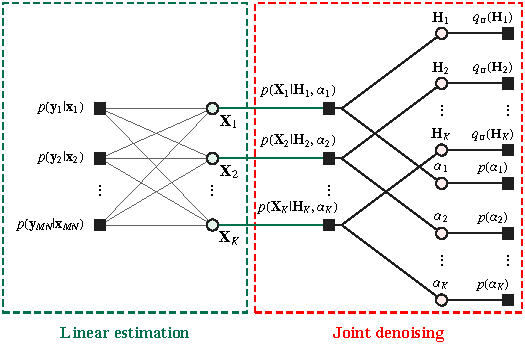
\includegraphics[width=\linewidth]{factor_graph.pdf}
\caption{Factor graph of \eqref{eq:working-posterior} using device blocks
$\mathbf X_k$ as variable nodes. Each likelihood factor depends on the corresponding
column entries from all device blocks. Circles and squares denote
variables and factors. The channel and activity prior branches are
adapted from \cite{cai2026}.}
\label{fig:receiver-structure}
\end{figure}

\subsection{Linear Estimation}
\label{sec:linear-estimation}

Following Turbo-CS \cite{ma2015}, we start by expressing the message to
the factor node $p(\mathbf y_j\mid\mathbf x_j)$ as
$\CN(\mathbf x_j;\mathbf x_j^{\rm pri},\gamma\I_{KN})$, where
$\mathbf x_j^{\rm pri}$ is the $j$th column of $\mathbf X^{\rm pri}$
and $\gamma>0$. Combining this message with the likelihood
$p(\mathbf y_j\mid\mathbf x_j)$ gives a Gaussian belief whose mean
and covariance are given by \cite{ma2017}:
\begin{align}
 \mathbf X_{\rm L}
 &=\mathbf X^{\rm pri}
 +\gamma\widehat{\mathbf A}^{\mathsf H}
 (\widehat\sigma^2\I_Q+\gamma\widehat{\mathbf A}\widehat{\mathbf A}^{\mathsf H})^{-1}
 (\mathbf Y-\widehat{\mathbf A}\mathbf X^{\rm pri}),
 \label{eq:linear-mean}\\
 \bm\Sigma_{\rm L}
 &=(\gamma^{-1}\I_{KN}+\widehat\sigma^{-2}\widehat{\mathbf A}^{\mathsf H}\widehat{\mathbf A})^{-1}.
 \label{eq:linear-variance}
\end{align}
Eqns.~\eqref{eq:linear-mean} and \eqref{eq:linear-variance} give, respectively,
the posterior mean matrix and per-column covariance from the linear MMSE
(LMMSE) estimator of $\mathbf X$. We further approximate the
covariance matrix using a shared scalar variance
$t_{\rm L}=\tr(\bm\Sigma_{\rm L})/(KN)$, resulting in a belief of the form
$\CN(\mathbf x_j;\mathbf x_{{\rm L},j},t_{\rm L}\I_{KN})$, where
$\mathbf x_{{\rm L},j}$ is the $j$th column of $\mathbf X_{\rm L}$.

The extrinsic message is proportional to the ratio of the above Gaussian
belief to the prior message. The variance $v_{\rm L}$ and mean matrix
$\mathbf R_{\rm L}$ are respectively given by
\begin{align}
 v_{\rm L}&=(t_{\rm L}^{-1}-\gamma^{-1})^{-1},
 \label{eq:linear-extrinsic}\\
 \mathbf R_{\rm L}&=v_{\rm L}
 \left(\frac{\mathbf X_{\rm L}}{t_{\rm L}}
       -\frac{\mathbf X^{\rm pri}}{\gamma}\right).
 \label{eq:linear-extrinsic-mean}
\end{align}
The extrinsic message flows rightward through the factor graph unchanged,
serving as the input to the joint denoiser, with $\mathbf R_k$ denoting the $k$th
device block of $\mathbf R_{\rm L}$ and $v=v_{\rm L}$.

\subsection{Joint Channel Estimation and Activity Detection}
\label{sec:joint-denoising}

For device $k$, the Gaussian message from the linear estimator,
with mean $\mathbf R_k$ and variance $v$, gives the local observation model
\begin{equation}
 \begin{gathered}
 \mathbf R_k=\alpha_k \mathbf H_k+\mathbf W_k,\\
 \vect(\mathbf W_k)\sim\CN(\mathbf0,v\I_D),
 \end{gathered}
 \label{eq:pseudo-awgn}
\end{equation}
where $\mathbf H_k\sim q_{\rm tr}$ and $D=MN^2$.

\subsubsection{Channel Estimation}
\label{sec:channel-estimation}

Under the active hypothesis $\alpha_k=1$, the Gaussian message
from the linear estimator has the form of the likelihood
$p(\mathbf R_k\mid\mathbf H_k,\alpha_k=1)$ in the AWGN model
\eqref{eq:pseudo-awgn}. Computing the conditional mean of $\mathbf H_k$
therefore amounts to MMSE denoising. The channel mean and a shared
average variance are approximated by
\begin{align}
 \mathbf F_k&\approx
 \E[\mathbf H_k\mid\mathbf R_k,\alpha_k=1],
 \label{eq:conditional-channel-integrals}\\
 \tau^{\rm post}&\approx\frac1{KD}\sum_{k=1}^K\tr\operatorname{Cov}
 (\vect(\mathbf H_k)\mid\mathbf R_k,\alpha_k=1).
 \label{eq:conditional-channel-variance}
\end{align}
Calculating the channel mean and shared average variance involves
high-dimensional integrals.

We approximate the channel prior by a Gaussian site
$\CN(\vect(\mathbf H_k);\vect(\mathbf E_k),\tau_k^{\rm ext}\I_D)$
\cite{vehtari2020}. Dividing the Gaussian belief,
with mean $\mathbf F_k$ and variance $\tau^{\rm post}$, by the input
likelihood gives the site parameters
\begin{align}
 \tau_k^{\rm ext}&=((\tau^{\rm post})^{-1}-v^{-1})^{-1},
 \label{eq:site-update}\\
 \mathbf E_k&=\tau_k^{\rm ext}\left(\frac{\mathbf F_k}{\tau^{\rm post}}-\frac{\mathbf R_k}{v}\right).
 \label{eq:site-mean}
\end{align}

\subsubsection{Activity Detection}
\label{sec:activity-detection}

Marginalizing over $\mathbf H_k$ in \eqref{eq:pseudo-awgn} yields the
likelihoods conditioned on $\alpha_k=1$ and $\alpha_k=0$, respectively:
\begin{align}
 q_{1,v}(\mathbf R)&=\E[\CN(\vect(\mathbf R);\vect(\mathbf H),v\I_D)],
 \label{eq:query-densities}\\
 q_{0,v}(\mathbf R)&=\CN(\vect(\mathbf R);\mathbf0,v\I_D).
 \label{eq:inactive-density}
\end{align}
The expectation is taken over $\mathbf H\sim q_{\rm tr}$.

The belief of $\alpha_k$ given $\mathbf R_k$ is a Bernoulli distribution
with parameter $p^\star(\mathbf R_k,v)$, where
\begin{equation}
 p^\star(\mathbf R,v)=\frac{\rho q_{1,v}(\mathbf R)}
 {(1-\rho)q_{0,v}(\mathbf R)+\rho q_{1,v}(\mathbf R)}.
 \label{eq:local-activity}
\end{equation}
We denote the approximation to $p^\star(\mathbf R_k,v)$ used in joint
estimation by $p_k$.

\subsubsection{Joint Estimation and Extrinsic Message}
\label{sec:joint-extrinsic}

Combining the site with the current Gaussian likelihood gives the
conditional channel variance and mean:
\begin{align}
 t_k&=\frac{\tau_k^{\rm ext}v}{\tau_k^{\rm ext}+v},
 \label{eq:conditional-moments}\\
 \mathbf H_k^{\rm post}&=\frac{\tau_k^{\rm ext}\mathbf R_k+v\mathbf E_k}{\tau_k^{\rm ext}+v}.
 \label{eq:conditional-channel-mean}
\end{align}

The approximate belief of $\mathbf X_k=\alpha_k\mathbf H_k$ is a
Bernoulli--Gaussian pdf \cite{liu2018}, with activity probability $p_k$
and a Gaussian active-channel component having mean
$\mathbf H_k^{\rm post}$ and covariance $t_k\I_D$.
The Gaussian projection gives the mean of $\mathbf X_k$ with respect
to the belief as
\begin{equation}
 \widehat{\mathbf X}_k=p_k\mathbf H_k^{\rm post}.
 \label{eq:mixture}
\end{equation}
The variances of the elements of $\mathbf X_k$ with respect to the belief
are averaged over all devices and channel coefficients to obtain
\begin{equation}
 \overline t_X=\frac1K\sum_k\left[
 p_kt_k+p_k(1-p_k)\frac{\norm{\mathbf H_k^{\rm post}}_F^2}{D}\right].
 \label{eq:joint-average-variance}
\end{equation}
Based on the above, the projected Gaussian belief is expressed as
$\CN(\vect(\mathbf X_k);\vect(\widehat{\mathbf X}_k),\overline t_X\I_D)$.

Finally, we calculate the message from the factor node
$p(\mathbf X_k\mid\mathbf H_k,\alpha_k)$ to the variable node
$\mathbf X_k$ as the ratio of the projected Gaussian belief to the
Gaussian message from the linear estimator. With $b=\overline t_X/v$, the extrinsic
variance and mean are respectively given by
\begin{align}
 \gamma_{\rm out}&=\frac{vb}{1-b},
 \label{eq:nonlinear-extrinsic}\\
 \mathbf X_{k,\rm out}&=\frac{\widehat{\mathbf X}_k-b\mathbf R_k}{1-b}.
 \label{eq:nonlinear-extrinsic-mean}
\end{align}
The extrinsic message in
\eqref{eq:nonlinear-extrinsic}--\eqref{eq:nonlinear-extrinsic-mean}
flows leftward through the factor graph unchanged, serving as the prior
message of the linear estimator in the next iteration, i.e.,
$\mathbf X^{\rm pri}=[\mathbf X_{1,\rm out}^{\mathsf T},\ldots,
\mathbf X_{K,\rm out}^{\mathsf T}]^{\mathsf T}$ and
$\gamma=\gamma_{\rm out}$.

\section{Learning Channel Denoising and Activity Detection}
\label{sec:learning}

In this section, we introduce score-based representations of the channel
mean and variance to circumvent the high-dimensional integrals in channel estimation.
We then apply denoising score matching for channel denoising and binary
classification for activity detection.

\subsection{Channel Mean Estimation with a Score-Based Generative Prior}
\label{sec:score-denoising}
\label{sec:channel-learning}

Under the active hypothesis in \eqref{eq:pseudo-awgn},
$\mathbf H\sim q_{\rm tr}$ is observed in independent proper complex
Gaussian noise with covariance $v\I_D$, where $v>0$.
Stacking the real and imaginary parts of $\vect(\mathbf H)$ and
$\vect(\mathbf R)$ into $\mathbf h_{\mathbb R}$ and $\mathbf u$,
respectively, we rewrite the AWGN observation model as
\begin{equation}
 \mathbf u=\mathbf h_{\mathbb R}+\sqrt{v/2}\,\bm\epsilon,
 \qquad \bm\epsilon\sim\mathcal N(\mathbf0,\I_{2D}).
 \label{eq:training-query}
\end{equation}

At fixed $v$, let $q_v^{\mathbb R}$ denote the density of $\mathbf u$.
For the model in \eqref{eq:training-query}, Tweedie's formula
\cite{efron2011,dytso2023} gives the conditional mean as
\begin{equation}
 \mathbf m_{\mathbb R}(\mathbf u,v)
 =\mathbf u+\frac v2\nabla_{\mathbf u}
       \log q_v^{\mathbb R}(\mathbf u),
 \label{eq:tweedie-mean}
\end{equation}
where $\nabla_{\mathbf u}\log q_v^{\mathbb R}$ is the first-order score
function of $q_v^{\mathbb R}$.

For a specific value of $v$, our goal is to learn a first-order score
network $\mathbf s_\theta(\cdot,v):\mathbb R^{2D}\to\mathbb R^{2D}$
parameterized by $\theta$ with the following score matching objective:
\begin{equation*}
 \min_\theta\;
 \E_{\mathbf u\sim q_v^{\mathbb R}}
 \left[\norm{\mathbf s_\theta(\mathbf u,v)
 -\nabla_{\mathbf u}\log q_v^{\mathbb R}(\mathbf u)}^2\right].
\end{equation*}
This objective cannot be directly used as the loss function since
$\nabla_{\mathbf u}\log q_v^{\mathbb R}(\mathbf u)$ is unknown.
The above objective has the same minimizers as the denoising score
matching objective \cite{vincent2011}, whose target is the conditional
Gaussian score $-2(\mathbf u-\mathbf h_{\mathbb R})/v$.

In practice, the score-based MMSE denoiser is required to operate across
a range of noise levels. We therefore combine the denoising score
matching objectives for different values of $v$ with weight $v/(4D)$
to establish a unified objective:
\begin{equation}
 \mathcal L_{\rm DSM}(\theta)=
 \E\left[\frac{v}{4D}
 \norm{\mathbf s_\theta(\mathbf u,v)
 +\frac2v(\mathbf u-\mathbf h_{\mathbb R})}^2\right].
 \label{eq:denoising-score-objective}
\end{equation}
The expectation is taken over the clean channels,
noise variances, and Gaussian noise.

We parameterize the score by a denoiser $\mathbf f_\theta(\mathbf u,v)$
as $\mathbf s_\theta=2(\mathbf f_\theta-\mathbf u)/v$.
Substituting this expression into \eqref{eq:denoising-score-objective}
yields
\begin{equation}
 \mathcal L_{\rm ch}(\theta)=
 \E\left[\frac{1}{Dv}
 \norm{\mathbf f_\theta(\mathbf u,v)-\mathbf h_{\mathbb R}}^2\right].
 \label{eq:first-loss}
\end{equation}
The conditional mean $\mathbf m_{\mathbb R}(\mathbf u,v)$ minimizes
this loss over all estimators of $\mathbf h_{\mathbb R}$ from
$(\mathbf u,v)$. Reshaping the real and imaginary outputs gives the
complex-valued estimate $\mathbf F_\theta(\mathbf R,v)$.

\subsection{Channel Variance Estimation}
\label{sec:conditional-error}

Likewise, the conditional covariance matrix
$\mathbf P_{\mathbb R}=\operatorname{Cov}(\mathbf h_{\mathbb R}\mid\mathbf u,v)$
can be obtained through the second-order Tweedie's formula
\cite{dytso2023} as
\begin{equation}
 \mathbf P_{\mathbb R}
 =\frac v2\I_{2D}+\frac{v^2}{4}
   \nabla_{\mathbf u}^2\log q_v^{\mathbb R}(\mathbf u).
 \label{eq:tweedie-covariance}
\end{equation}

Differentiating \eqref{eq:tweedie-mean} with respect to $\mathbf u$
at fixed $v$ gives the following compact expressions for the covariance
in \eqref{eq:tweedie-covariance} and its normalized trace:
\begin{align}
 \mathbf P_{\mathbb R}&=\frac v2\mathbf J_m,
 \label{eq:mean-derivative-covariance}\\
 \tau^\star&=\frac{v}{2D}\operatorname{div}\mathbf m_{\mathbb R}.
 \label{eq:mean-derivative-variance}
\end{align}
Here $\mathbf J_m=\partial\mathbf m_{\mathbb R}/\partial\mathbf u$
denotes the Jacobian of $\mathbf m_{\mathbb R}$, and $\tau^\star$ is the
average conditional variance per complex coordinate.
This suggests that the average conditional variance can be estimated
by computing the divergence of the trained denoiser $\mathbf f_\theta$
\cite{manor2024}.

The divergence is estimated by a Monte Carlo method \cite{metzler2016},
using $L_z$ independent random sign vectors $\mathbf z_\ell$ with
$\E[\mathbf z_\ell\mathbf z_\ell^{\mathsf T}]=\I_{2D}$.
Central finite differences along $\mathbf w_\ell=\sqrt{v/2}\,\mathbf z_\ell$,
with step $\delta_{\rm FD}>0$, give an estimate of the average conditional variance:
\begin{equation}
 \widehat\tau_\theta(\mathbf R,v)
 =\frac{1}{2\delta_{\rm FD} D L_z}\sum_{\ell=1}^{L_z}
       \mathbf w_\ell^{\mathsf T}\Delta_\ell \mathbf f_\theta,
 \label{eq:derivative-trace}
\end{equation}
where $\Delta_\ell \mathbf f_\theta
 =\mathbf f_\theta(\mathbf u+\delta_{\rm FD}\mathbf w_\ell,v)
 -\mathbf f_\theta(\mathbf u-\delta_{\rm FD}\mathbf w_\ell,v)$.

\subsection{Activity Probability Estimation Based on Density Ratios}
\label{sec:density-ratio}

The density ratio $q_{1,v}/q_{0,v}$ can be estimated from samples with
binary labels $a\in\{0,1\}$, where
$q_{1,v}$ and $q_{0,v}$ are the class-conditional densities at fixed $v$
\cite{menon2016}. For the activity prior $\rho$, Bayes' rule implies
\begin{equation}
 \log\frac{p^\star(\mathbf R,v)}{1-p^\star(\mathbf R,v)}
 =\log\frac{\rho}{1-\rho}
  +\log\frac{q_{1,v}(\mathbf R)}{q_{0,v}(\mathbf R)}.
 \label{eq:activity-log-odds}
\end{equation}

For training, we set $\Pr(a=1)=1/2$.
Samples from the active class $a=1$ are generated as
$\mathbf R=\mathbf H+\mathbf W$, with $\mathbf H\sim q_{\rm tr}$,
whereas samples from the inactive class $a=0$ are generated as
$\mathbf R=\mathbf W$.
The noise satisfies $\vect(\mathbf W)\sim\CN(\mathbf0,v\I_D)$
independently of $\mathbf H$, and both classes use the same sampling
distribution of $v$.
We train the classifier with parameters $\phi$ by minimizing the
binary cross-entropy loss
\begin{equation}
 \mathcal L_{\rm act}(\phi)=
 \E[\log(1+e^{z_\phi})-a z_\phi],
 \label{eq:classifier-loss}
\end{equation}
where $z_\phi=z_\phi(\mathbf R,v,\mathbf F_\theta(\mathbf R,v))$.
For the balanced training distribution, the Bayes-optimal logit is
\begin{equation}
 z^\star(\mathbf R,v)=
       \log\frac{q_{1,v}(\mathbf R)}{q_{0,v}(\mathbf R)}.
 \label{eq:ideal-logit}
\end{equation}

Given a trained classifier $z_\phi$, we use
$\ell_k=z_\phi(\mathbf R_k,v,\mathbf F_k)$ as an estimate of the log
likelihood ratio, where $\mathbf F_k=\mathbf F_\theta(\mathbf R_k,v)$.
Substituting this estimate into \eqref{eq:activity-log-odds} gives the
activity update
\begin{equation}
 p_k=\sigmoid(\logit\rho+\ell_k),
 \label{eq:activity-probability}
\end{equation}
where $\logit a=\log[a/(1-a)]$ and $\sigmoid b=(1+e^{-b})^{-1}$.

\section{GP-MP Algorithm}
\label{sec:overall}

\subsection{Overall Algorithm}
\label{sec:schedule}

The trained denoiser provides the channel mean
$\mathbf F_k=\mathbf F_\theta(\mathbf R_k,v)$, while the variance
estimate $\widehat\tau_k=\widehat\tau_\theta(\mathbf R_k,v)$ is given by
\eqref{eq:derivative-trace}.
Averaging $\widehat\tau_k$ over devices and applying the positive lower
bound $\tau_{\min}$ gives $\tau^{\rm post}$.
The trained activity classifier provides $p_k$ through
\eqref{eq:activity-probability}.

Fig.~\ref{fig:learned-receiver} illustrates the generative-prior
message-passing (GP-MP) receiver, in which GPJD uses the trained
denoiser and activity classifier, while MFLE is derived analytically.

\begin{figure*}[!t]
\centering
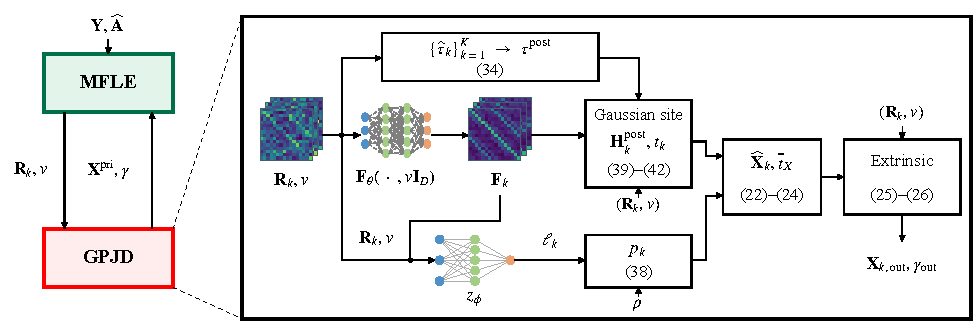
\includegraphics[width=0.92\textwidth]{learned_receiver.pdf}
\caption{Message exchange between MFLE and GPJD, with an expanded view of GPJD.
The denoising illustration follows \cite{cai2026}.}
\label{fig:learned-receiver}
\end{figure*}

The phases are either known or estimated once before MP and remain
fixed during the iterations. For initialization, $\widehat P_H$ is the
normalized training-channel power, computed by averaging
$\norm{\mathbf H}_F^2/D$ over the training channels.

Algorithm~\ref{alg:gp-mp-ccd} presents the pseudocode for GP-MP.

\begin{figure}[!t]
\centering
\begin{minipage}{\linewidth}
\small
\refstepcounter{algorithm}\label{alg:gp-mp-ccd}
\hrule\vspace{3pt}
\textbf{Algorithm \thealgorithm}\enspace GP-MP for JADCE\par
\vspace{3pt}\hrule\vspace{3pt}
\begin{algorithmic}[1]
 \Require $\mathbf Y$, $\{\mathbf p_{qk}\}$, available phases, $\rho$, trained
 $\mathbf f_\theta$ and $z_\phi$.
 \Ensure $\{s\widehat{\mathbf X}_k,s\mathbf H_k^{\rm post},p_k,\widehat\alpha_k\}_{k=1}^K$.
 \State Estimate $\widehat\sigma^2$; estimate any unknown phases once as described in
 Section~\ref{sec:phase-estimation}.
 \State Construct $\widehat{\mathbf A}$ using fixed phases; normalize $\mathbf Y$ and $\widehat\sigma^2$ as in Section~\ref{sec:frontend}.
 \State Compute the SVD of $\widehat{\mathbf A}$; draw one random sign vector
 per device and reuse it across iterations.
 \State Initialize $\mathbf X^{{\rm pri},(0)}\gets\mathbf0$,
 $\gamma^{(0)}\gets\rho\widehat P_H$.
 \State Initialize $\mathbf E_k\gets\mathbf0$, $\tau_k^{\rm ext}\gets1$,
 $\kappa^{(1)}\gets1$.
 \For{$i=1,\ldots,I_{\max}$}
  \Statex \hspace{\algorithmicindent}\textit{\% MFLE}
  \State Update $\mathbf R_{{\rm L},k}$ and $v_{\rm L}$ by
  \eqref{eq:linear-mean}--\eqref{eq:linear-extrinsic-mean}, using
  \eqref{eq:linear-fraction}--\eqref{eq:linear-svd-extrinsic}.
  \State $\mathbf R_k\gets\mathbf R_{{\rm L},k}$, $\bar v\gets v_{\rm L}$;
  apply \eqref{eq:input-damping}--\eqref{eq:input-variance-damping} for $i\geq2$.
  \State $v\gets\kappa^{(i)}\bar v$.
  \Statex \hspace{\algorithmicindent}\textit{\% GPJD}
  \State $\mathbf F_k\gets\mathbf F_\theta(\mathbf R_k,v)$.
  \State Compute $\widehat\tau_k$ and $p_k$ by \eqref{eq:derivative-trace}
  and \eqref{eq:activity-probability}.
  \State Average $\widehat\tau_k$ over $k$ to obtain $\tau^{\rm post}$.
  \State Apply the lower bound $\tau_{\min}$ to $\tau^{\rm post}$.
  \If{$\tau^{\rm post}<v$}
   \State Update $\mathbf E_k$ and $\tau_k^{\rm ext}$ by
   \eqref{eq:site-update}--\eqref{eq:site-mean}.
  \EndIf
  \State Update $\mathbf H_k^{\rm post}$ and $t_k$ by
  \eqref{eq:conditional-moments}--\eqref{eq:conditional-channel-mean}.
  \State Update $\widehat{\mathbf X}_k$ and $\overline t_X$ by
  \eqref{eq:mixture} and \eqref{eq:joint-average-variance}.
  \State Update $\kappa^{(i+1)}$ as in Section~\ref{sec:variance-update}.
  \State Compute $\mathbf X_{k,\rm out}$ and $\gamma_{\rm out}$ by
  \eqref{eq:nonlinear-extrinsic}--\eqref{eq:nonlinear-extrinsic-mean} with clipping.
  \State $\mathbf X_k^{{\rm pri},(i)}\gets\mathbf X_{k,\rm out}$,
  $\gamma^{(i)}\gets\gamma_{\rm out}$; apply
  \eqref{eq:output-damping}--\eqref{eq:output-variance-damping} for $i\geq2$.
  \State Update the stopping history.
  \If{the stopping conditions in Section~\ref{sec:stopping-criteria} hold}
   \State \textbf{break}
  \EndIf
 \EndFor
 \State $\widehat\alpha_k\gets\mathbf1\{p_k\geq1/2\}$.
 \State \Return $\{s\widehat{\mathbf X}_k,s\mathbf H_k^{\rm post},p_k,\widehat\alpha_k\}_{k=1}^K$.
\end{algorithmic}
\vspace{3pt}\hrule
\end{minipage}
\end{figure}

\subsection{Parameter Estimation and Numerical Implementation}
\label{sec:frontend}
\label{sec:phase-estimation}
\label{sec:variance-update}
\label{sec:damping}

For noise estimation, the Wax--Kailath minimum description length
(MDL) criterion \cite{wax1985,nadakuditi2008} is used to estimate the
signal covariance rank $\widehat r_{\rm s}$ based on the eigenvalues
$\lambda_1\geq\cdots\geq\lambda_M$ of the sample covariance matrix.
Let $\mathbf y_{qr}$ denote column $r$ of $\mathbf Y_q$ and
$N_{\rm s}=QN>M\geq2$. The sample covariance and noise estimate are
\begin{align}
 \widehat{\mathbf R}_y&=\frac1{N_{\rm s}}\sum_{q,r}
 \mathbf y_{qr}\mathbf y_{qr}^{\mathsf H},
 \label{eq:sample-spatial-covariance}\\
 \widehat\sigma^2&=\frac{\sum_{i=\widehat r_{\rm s}+1}^{M}\lambda_i}
 {M-\widehat r_{\rm s}}.
 \label{eq:noise-estimation}
\end{align}
This estimate assumes a low-rank signal covariance and is held fixed
during MP.

For phase estimation, the observations are stacked into the matrix
$\mathbf Y_{\rm s}=[\mathbf Y_0,\ldots,\mathbf Y_{Q-1}]^{\mathsf T}
\in\mathbb C^{QN\times M}$.
The dominant line-of-sight component of the default NTN-TDL-D
channel motivates a single-path approximation of each device's
channel for estimating its common Doppler shift. Absorbing the common scalar
phase into the path gain gives
\begin{equation}
 [\mathbf h_k^{\rm p}(d,\nu)]_{qN+r}
 =e^{\mathrm j2\pi\nu qT_{\rm frame}}
 [\mathbf G_0(d,\nu)\mathbf p_{qk}]_r,
 \label{eq:phase-atom}
\end{equation}
where $\mathbf G_0(d,\nu)=e^{-\mathrm j2\pi c_1d^2}\mathbf G(d,\nu;0)$.

With $\mathbf h_k^{\rm p}=\mathbf h_k^{\rm p}(d_k,\nu_k)$, the
observations can be expressed as
$\mathbf Y_{\rm s}\approx\sum_k\mathbf h_k^{\rm p}\mathbf b_k^{\mathsf T}
+\mathbf W_{\rm s}$.
This observation model is complemented by independent Gaussian priors
over the gains, $\mathbf b_k\sim\CN(\mathbf0,\gamma_k\I_M)$,
$\gamma_k\geq0$.
Phase estimation is formulated as the minimization of the negative log
marginal likelihood \cite{tipping2003}, obtained by integrating out
the gains:
\begin{align}
 \mathbf S&=\widehat\sigma^2\I_{QN}
 +\sum_k\gamma_k\mathbf h_k^{\rm p}\mathbf h_k^{{\rm p},\mathsf H},
 \label{eq:phase-covariance}\\
 \mathcal L&=\log\det\mathbf S+
 \frac1M\tr(\mathbf Y_{\rm s}^{\mathsf H}\mathbf S^{-1}\mathbf Y_{\rm s}).
 \label{eq:phase-objective}
\end{align}
The objective $\mathcal L$ is minimized by coordinate updates, with
each $\gamma_k$ solved for analytically and $(d_k,\nu_k)$ refined
using L-BFGS-B
\cite{zhu1997}.

The estimated Doppler determines $\widehat\beta_k$ and
$\widehat{\mathbf A}$ through
\eqref{eq:twc-frame-channel}--\eqref{eq:effective-pilot}.

To match the scale used for denoiser training, the channel and
observation quantities $(\mathbf H_k,\mathbf X_k,\mathbf Y,\mathbf W)$
are divided by the root mean square $s$ of the training-channel
entries, and the noise variance is divided by $s^2$.
The same symbols denote the normalized quantities.

In each iteration, the mean and variance updates are damped using a
linear combination of the current update and the previous damped
message \cite{rangan2019}.
With damping factor $\eta\in(0,1]$, the input messages to GPJD for
$i\geq2$ are
\begin{align}
 \mathbf R_k^{(i)}&=(1-\eta)\mathbf R_k^{(i-1)}+\eta \mathbf R_{{\rm L},k}^{(i)},
 \label{eq:input-damping}\\
 \bar v^{(i)}&=(1-\eta)\bar v^{(i-1)}+\eta v_{\rm L}^{(i)}.
 \label{eq:input-variance-damping}
\end{align}
At iteration $i$, GPJD uses $v^{(i)}=\kappa^{(i)}\bar v^{(i)}$.
After joint denoising, the update of the input variance follows from
minimizing the expected Gaussian negative log likelihood, with the current
approximate posterior held fixed \cite{vila2013}.
Setting the derivative with respect to the variance to zero yields
\begin{equation}
 v_{\rm tar}=\frac{1}{KD}\sum_{k=1}^K
 \norm{\mathbf R_k-\widehat{\mathbf X}_k}_F^2+\overline t_X.
 \label{eq:query-variance-target}
\end{equation}
The next scaling factor $\kappa^{(i+1)}$ is obtained by averaging
$\kappa^{(i)}$ and $v_{\rm tar}^{(i)}/\bar v^{(i)}$ with weights
$1-\eta$ and $\eta$, respectively.

The input to MFLE is damped in a similar manner.
In the feedback updates
\eqref{eq:nonlinear-extrinsic}--\eqref{eq:nonlinear-extrinsic-mean},
$b=\overline t_X/v$ is clipped to $[\varepsilon,1-\varepsilon]$,
where $0<\varepsilon<1/2$.
With the same damping factor, the feedback messages for $i\geq2$ are
\begin{align}
 \mathbf X_k^{{\rm pri},(i)}
 &=(1-\eta)\mathbf X_k^{{\rm pri},(i-1)}+\eta \mathbf X_{k,\rm out}^{(i)},
 \label{eq:output-damping}\\
 \gamma^{(i)}
 &=(1-\eta)\gamma^{(i-1)}+\eta\gamma_{\rm out}^{(i)}.
 \label{eq:output-variance-damping}
\end{align}

\subsection{Computational Complexity Analysis}
\label{sec:complexity}

With precomputed chirp factors, $L$ AFDM frames require at most
$LC_{\rm FFT}(N)+2LN$ complex multiplications
\cite{bemani2022}, where $C_{\rm FFT}(n)$ is the cost of an
$n$-point fast Fourier transform (FFT) or inverse FFT. For the same $LN$ useful symbols,
rectangular-pulse OTFS without transmit windowing requires
$NC_{\rm FFT}(L)$ after cancelling the consecutive discrete Fourier transform (DFT)
and inverse DFT operations
\cite{zou2021otfs}.

The computational complexity of the receiver is primarily determined
by the operations in MFLE and GPJD, together with parameter estimation.
With fixed phases and $Q\leq KN$, MFLE can be implemented using the
singular value decomposition (SVD),
$\widehat{\mathbf A}=\mathbf U\diag(s_1,\ldots,s_Q)\mathbf V^{\mathsf H}$,
which is reused across iterations. Here $s_a$ are the singular values,
and the scalar updates in
\eqref{eq:linear-variance}--\eqref{eq:linear-extrinsic} can be written as
\begin{align}
 f_{\rm L}&=\frac{1}{KN}\sum_{a=1}^{Q}
 \frac{\gamma s_a^2}{\widehat\sigma^2+\gamma s_a^2},
 \label{eq:linear-fraction}\\
 t_{\rm L}&=\gamma(1-f_{\rm L}),
 \label{eq:linear-svd-variance}\\
 v_{\rm L}&=\frac{t_{\rm L}}{f_{\rm L}}.
 \label{eq:linear-svd-extrinsic}
\end{align}
Here $\mathbf R_{\rm L}=\mathbf X^{\rm pri} +(\mathbf X_{\rm L}-\mathbf
X^{\rm pri})/f_{\rm L}$.

For each block, the SVD and noise-variance estimation require
$O(KNQ^2)$ and $O(QNM^2+M^3)$ operations, respectively.
The phase-estimation cost is denoted by $C_{\rm phase}$, with
$C_{\rm phase}=0$ for known phases.

For each iteration, the MFLE transformations involve $O(QKMN^2)$
operations, while the spatial covariance operations and matrix
factorizations require $O(KM^2N^2)$ and $O(M^3)$ operations,
respectively. The per-device costs of a forward pass through the
denoiser and classifier are denoted by $C_\theta$ and $C_\phi$,
respectively. Each GPJD update evaluates the denoiser $1+2L_z$ times
and the classifier once per device. Consequently, these forward
passes require $K[(1+2L_z)C_\theta+C_\phi]$ operations.

Overall, the online complexity for $I$ iterations is
$O(C_{\rm phase}+QNM^2+M^3+KNQ^2+I C_{\rm iter})$, where
$C_{\rm iter}$ denotes the total per-iteration cost.
The pilot matrix, SVD factors, channel messages, and spatial
covariances require $O(QKN+KMN^2+KM^2)$ memory.

\section{Simulation Results}
\label{sec:simulations}

\subsection{Simulation Settings}
\label{sec:simulation-settings}

\subsubsection{Channel Dataset and System Parameters}
The default system parameters are listed in
Table~\ref{tab:simulation-parameters}. Devices are uniformly distributed
within the satellite beam, and their delays, Doppler shifts, and array
responses follow the satellite-device geometry. Large-scale effects are
compensated. Channels follow the NTN-TDL-D profile \cite{shen2025},
with delay spread uniformly distributed over $[30,50]$~ns. The
line-of-sight gain has fixed amplitude and uniform phase, and the
diffuse gains are proper complex Gaussian.
We generate $50{,}000$ training channels and $5{,}000$ validation
channels of size $16\times16\times16$.

For $Q\leq KN$, the pilots are constructed from distinct DFT rows
$r_q\in\{0,\ldots,KN-1\}$, with a column permutation
$\{c_{kn}\}_{k,n}$ of the same set and independent phases
$\phi_{kn}\sim\mathcal U[0,2\pi)$:

\begin{equation}
 [\mathbf p_{qk}]_n=\sqrt{\frac{E_p}{N}}
 e^{-\mathrm j2\pi r_qc_{kn}/(KN)}e^{\mathrm j\phi_{kn}},
 \label{eq:pilot}
\end{equation}
with $\sum_{n=0}^{N-1}|[\mathbf p_{qk}]_n|^2=E_p$.

The received SNR is defined as the average signal power over the $QMN$
entries of $\mathbf A\mathbf X$ divided by $\sigma^2$. We set
$\sigma^2$ separately for each scene to obtain the specified SNR.

\begin{table}[!t]
\caption{Simulation Parameters}
\label{tab:simulation-parameters}
\centering
\small
\begin{tabular}{@{}ll@{}}
\toprule
Parameter & Value \\
\midrule
Carrier frequency $f_c$ & $2$~GHz \\
Satellite altitude & $600$~km \\
Beam radius & $128$~km \\
Minimum elevation angle & $30^\circ$ \\
UPA dimensions $M_y\times M_z$ & $4\times4$ \\
Array element spacing $d_y,d_z$ & $\lambda/2$ \\
Number of chirp subcarriers $N$ & $16$ \\
Subcarrier spacing $\Delta f$ & $30$~kHz \\
Chirp parameters $(c_1,c_2)$ & $(7/32,1/320)$ \\
CPP length $N_{\rm CPP}$ & $336$ \\
Differential-delay range & $[0,699]~\mu$s \\
Doppler-shift range & $[-41,41]$~kHz \\
Power delay profile & NTN-TDL-D \\
Delay spread & $[30,50]$~ns \\
Rician factor & $11.707$~dB \\
Default $(K,Q,p)$ & $(40,16,0.1)$ \\
\bottomrule
\end{tabular}
\end{table}

\subsubsection{Network Architectures and Training}
\label{sec:network-settings}
\label{sec:training-settings}
The denoiser uses the RefineNet \cite{lin2017} variant in
\cite{song2019}, with $2M$ real and imaginary input maps over
$N\times N$ DAFT coordinates.
Each stage contains two residual blocks, each with two
$3\times3$ convolutions, conditional instance normalization, and
exponential linear unit (ELU) activations.
The stage outputs are combined by four refinement blocks that restore
the spatial resolution, with $3\times3$ convolutions at the network
input and output. Table~\ref{tab:network-architectures} lists the channel
widths and spatial resolutions of both networks.

\begin{table}[!t]
\caption{Network Architectures}
\label{tab:network-architectures}
\centering
\small
\setlength{\tabcolsep}{3pt}
\begin{tabular}{@{}lcc@{}}
\toprule
Layer or stage & Channels & Map size \\
\midrule
\multicolumn{3}{@{}l}{\textit{Channel denoiser}} \\
Input convolution & $128$ & $N\times N$ \\
Residual stage 1 & $128$ & $N\times N$ \\
Residual stage 2 & $256$ & $N/2\times N/2$ \\
Residual stage 3 (dilation 2) & $256$ & $N/2\times N/2$ \\
Residual stage 4 (dilation 4) & $256$ & $N/2\times N/2$ \\
Refinement blocks 1--2 & $256,256$ & $N/2\times N/2$ \\
Refinement block 3 & $128$ & $N/2\times N/2$ \\
Refinement block 4 & $128$ & $N\times N$ \\
Output convolution & $2M$ & $N\times N$ \\
\midrule
\multicolumn{3}{@{}l}{\textit{Activity classifier}} \\
Convolutional stage 1 & $64$ & $N\times N$ \\
Convolutional stage 2 & $128$ & $N/2\times N/2$ \\
Convolutional stage 3 & $128$ & $N/4\times N/4$ \\
Fully connected layers & $128,1$ & --- \\
\bottomrule
\end{tabular}
\end{table}

Noise conditioning uses an embedding of $\log(v)/5$, formed by two
$64$-unit fully connected layers with sigmoid-weighted linear unit
(SiLU) activations and linearly projected to the normalization layers.
The denoiser also adopts the preconditioning in \cite{karras2022}:

\begin{equation}
 \begin{aligned}
 \mathbf f_\theta(\mathbf u,v)
 &=c_{\rm skip}(v)\mathbf u+c_{\rm out}(v)
   \mathbf g_\theta(c_{\rm in}(v)\mathbf u,v),\\
 c_{\rm in}(v)&=(\sigma_{\rm d}^2+v/2)^{-1/2},\\
 c_{\rm skip}(v)&=\frac{\sigma_{\rm d}^2}{\sigma_{\rm d}^2+v/2},\\
 c_{\rm out}(v)&=\left(\frac{\sigma_{\rm d}^2 v/2}
 {\sigma_{\rm d}^2+v/2}\right)^{1/2}.
 \end{aligned}
 \label{eq:mean-preconditioning}
\end{equation}

Here $\sigma_{\rm d}^2=1/2$ is the nominal variance per real coordinate after
normalization, and $\mathbf g_\theta$ is the RefineNet described above.

The classifier estimates the log likelihood ratio from $4M$ real and
imaginary maps of $\mathbf R$ and $\mathbf F_\theta(\mathbf R,v)$,
scaled by $\sqrt{2/(1+v)}$, together with five scalars:
$\log(v)/5$, logarithmic transforms of input/output/residual energies
normalized by $Dv$, and a sign-preserving logarithmic transform of the
real inner product normalized by $Dv$.
Its three convolutional stages each contain two $3\times3$ convolutions
with SiLU activations and padding $1$. Downsampling uses stride $2$ in
the first convolution of stages~2--3; the remaining convolutions use
stride $1$.
Noise conditioning is provided by a $64$-unit fully connected SiLU
embedding of $\log(v)/5$, whose linear projections are added to the
stage outputs. The flattened features and five scalars are combined by
the fully connected layers in Table~\ref{tab:network-architectures},
with SiLU between them, to produce one logit per device.

We train the denoiser by minimizing \eqref{eq:first-loss} with the
preconditioning in \eqref{eq:mean-preconditioning}. The variance $v$
is sampled uniformly on a logarithmic scale over $[10^{-3},10^2]$.
We use Adam for $200$ epochs with batch size $64$, initial learning
rate $10^{-4}$, and exponential moving average decay $0.999$.
STMP uses the same clean channels and number of epochs.

With the denoiser fixed, we train the classifier using
\eqref{eq:classifier-loss} for $100$ epochs, with batch size $32$
and initial learning rate $3\times10^{-4}$. For both networks, we select
the model with the lowest validation loss.

\subsubsection{Compared Receivers}
\label{sec:compared-receivers}
We compare GP-MP with five baselines. GP-MP-EP uses estimated phases;
the other configurations use known phases:
\begin{itemize}[leftmargin=*,topsep=2pt,itemsep=2pt,parsep=0pt]

\item \textbf{STMP:} We adapt STMP \cite{cai2026} to the multi-frame
AFDM model, retaining its white-noise-trained first- and second-order
score networks for conditional mean and variance estimation. We replace
its Gaussian-message-based activity-probability update with a learned
density-ratio estimator trained using the corresponding first-order network.
\begin{samepage}
\item \textbf{Simultaneous orthogonal matching pursuit (SOMP)}
\cite{TroppGilbertStrauss2006SOMP}: This method selects dictionary atoms
shared by the receive antennas and estimates their coefficients by
least squares. We use an integer delay--Doppler dictionary
and select up to $64$ atoms.
\par
\end{samepage}
\item \textbf{GAMP-SBL:} This method uses generalized approximate message
passing in sparse Bayesian learning \cite{ZhangFanHaoQuan2023GAMPSBL}.
Our implementation uses the integer delay--Doppler dictionary,
shares row precisions across receive antennas, and allows up to
$1{,}000$ iterations.
\item \textbf{GNN-ASPL:} This method alternates AMP-based channel estimation
with adaptive sparsity pattern learning using a graph neural network
\cite{ding2026}. It uses the same integer delay--Doppler dictionary and
a $10$-layer network.
\item \textbf{Off-grid SBL:} In addition to the channel coefficients,
this method estimates continuous delay and Doppler offsets through a
first-order linear approximation of the dictionary
\cite{WeiEtAl2022OffgridSBL}. We allow up to $120$ iterations.
For the SNR comparison, the $7$, $13$, and $25$ Doppler grid points
are paired with $12$, $24$, and $48$ retained candidates per device
and $48$, $96$, and $192$ offset candidates per iteration, respectively;
all three configurations use $112$ delay grid points.
\end{itemize}

\subsubsection{Evaluation Settings and Metrics}
\label{sec:receiver-settings}
\label{sec:stopping-criteria}
Phase estimation in GP-MP-EP covers $d\in[0,N)$ and
$|\nu|\leq\nu_{\max}$, where $\nu_{\max}$ is the channel model's Doppler
bound. Pilot correlations over $128$ phase bins identify three coarse
candidates. The Doppler values corresponding to each candidate phase
within this bound form the initial search set, from which the best
$12$ are refined by at most $25$ L-BFGS-B iterations per candidate.

All receivers estimate the noise variance from the observations.
STMP and GP-MP use an activity threshold of $0.5$ and default damping factors
of $0.2$ and $0.4$, respectively.
Their iterations are bounded by $I_{\min}=60$ and $I_{\max}=600$,
with a relative-change tolerance of $5\times10^{-4}$.
After $I_{\min}$ iterations, convergence is assessed from the stability
of channel and activity estimates and the consistency of variance
updates.
\ifdefined\FullManuscript
The complete stopping checks and tolerances are given in
Appendix~\ref{app:implementation-settings}.
\fi

GP-MP uses $L_z=1$ and $\delta_{\rm FD}=10^{-2}$ in
\eqref{eq:derivative-trace}. The average conditional variance has a
lower bound $\tau_{\min}=10^{-4}$.

The evaluation protocol specifies $1{,}000$ Monte Carlo trials per
operating point.
\ifdefined\FullManuscript
Appendix~\ref{app:evaluation-protocol} gives the evaluation protocol.
\fi

For scenes $e\in\mathcal T$, the normalized mean-squared error (NMSE)
is the total squared Frobenius error between
$\widehat{\mathbf X}_{ek}$ and $\mathbf X_{ek}$ divided by the total
squared Frobenius norm of $\mathbf X_{ek}$. Both totals include all
scenes in $\mathcal T$ and all $K$ devices;
the ratio is expressed in decibels. For channel denoising, the same
metric uses $\mathbf H$ in place of $\mathbf X$ and is accumulated
over individual channel samples. The activity error rate (AER) is the
total number of missed detections and false alarms divided by
$K|\mathcal T|$.

\begin{figure}[!t]
\centering
\makebox[\columnwidth][c]{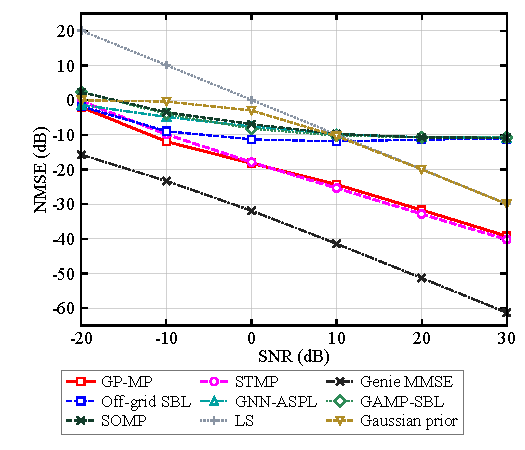
\includegraphics[width=88.9mm]{channel_denoising.pdf}}
\caption{Channel denoising under AWGN with known variance.}
\label{fig:cstmp-denoising}
\end{figure}

\begin{table}[!t]
\caption{Activity Detection Performance and Iteration-Limit Rates}
\label{tab:activity-evidence}
\centering
\small
\setlength{\tabcolsep}{2pt}
\begin{tabular}{@{}rcccccccc@{}}
\toprule
& \multicolumn{4}{c}{STMP}
& \multicolumn{4}{c}{GP-MP} \\
\cmidrule(lr){2-5}\cmidrule(l){6-9}
& \multicolumn{2}{c}{Gaussian} & \multicolumn{2}{c}{Density ratio}
& \multicolumn{2}{c}{Gaussian} & \multicolumn{2}{c}{Density ratio} \\
\cmidrule(lr){2-3}\cmidrule(lr){4-5}\cmidrule(lr){6-7}\cmidrule(l){8-9}
\shortstack{SNR\\(dB)} & \shortstack{AER\\(\%)} & \shortstack{Limit\\(\%)}
& \shortstack{AER\\(\%)} & \shortstack{Limit\\(\%)}
& \shortstack{AER\\(\%)} & \shortstack{Limit\\(\%)}
& \shortstack{AER\\(\%)} & \shortstack{Limit\\(\%)} \\
\midrule
$-4$ & $9.225$ & $2$ & $0.525$ & $0$ & $44.575$ & $63$ & $0.200$ & $0$ \\
$-2$ & $7.875$ & $3$ & $0.225$ & $0$ & $43.475$ & $55$ & $0.125$ & $0$ \\
$0$ & $6.375$ & $2$ & $0.100$ & $0$ & $40.975$ & $46$ & $0.075$ & $0$ \\
$2$ & $5.550$ & $1$ & $0.050$ & $0$ & $36.750$ & $31$ & $0.025$ & $0$ \\
$4$ & $4.800$ & $1$ & $0.025$ & $0$ & $32.050$ & $19$ & $0.025$ & $0$ \\
$6$ & $4.225$ & $0$ & $0.025$ & $0$ & $27.425$ & $11$ & $0.025$ & $0$ \\
\bottomrule
\end{tabular}
\end{table}

\begin{figure}[!t]
\centering
\makebox[\columnwidth][c]{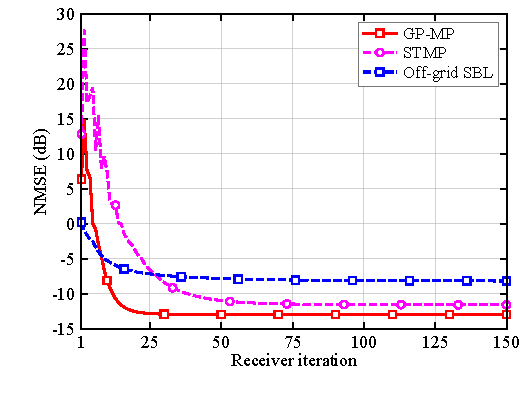
\includegraphics[width=88.9mm]{convergence.pdf}}
\caption{NMSE versus iteration at $0$~dB, with $K=40$, $Q=16$,
and $p=0.1$.}
\label{fig:cstmp-convergence}
\end{figure}

\begin{figure}[!t]
\centering
\makebox[\columnwidth][c]{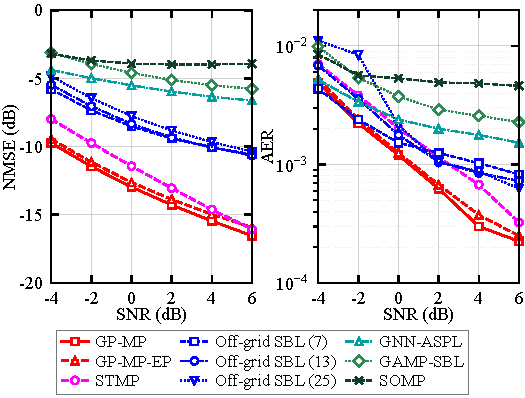
\includegraphics[width=88.9mm]{snr_comparison.pdf}}
\caption{Channel NMSE and AER versus SNR with $K=40$, $Q=16$,
and $p=0.1$.}
\label{fig:cstmp-snr}
\end{figure}

\begin{figure}[!t]
\centering
\makebox[\columnwidth][c]{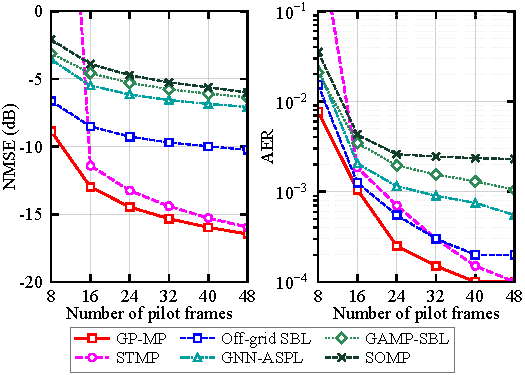
\includegraphics[width=88.9mm]{pilot_frames.pdf}}
\caption{Channel NMSE versus the number of pilot frames at
$0$~dB, with $K=40$ and $p=0.1$.}
\label{fig:cstmp-pilots}
\end{figure}

\begin{figure}[!t]
\centering
\makebox[\columnwidth][c]{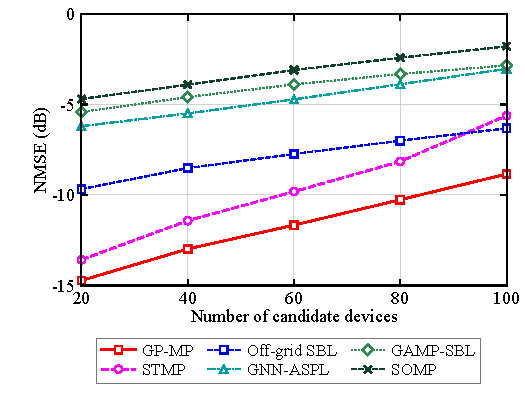
\includegraphics[width=88.9mm]{user_count.pdf}}
\caption{Channel NMSE versus the number of candidate devices
at $0$~dB, with $Q=16$ and $p=0.1$.}
\label{fig:cstmp-users}
\end{figure}

\begin{figure}[!t]
\centering
\makebox[\columnwidth][c]{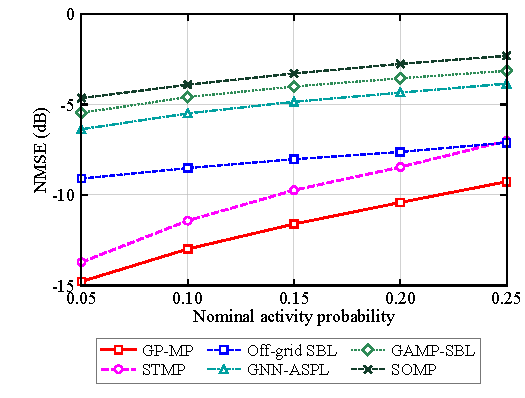
\includegraphics[width=88.9mm]{activity_probability.pdf}}
\caption{Channel NMSE versus nominal activity probability at
$0$~dB, with $K=40$ and $Q=16$.}
\label{fig:cstmp-activity}
\end{figure}

\begin{figure*}[!t]
\centering
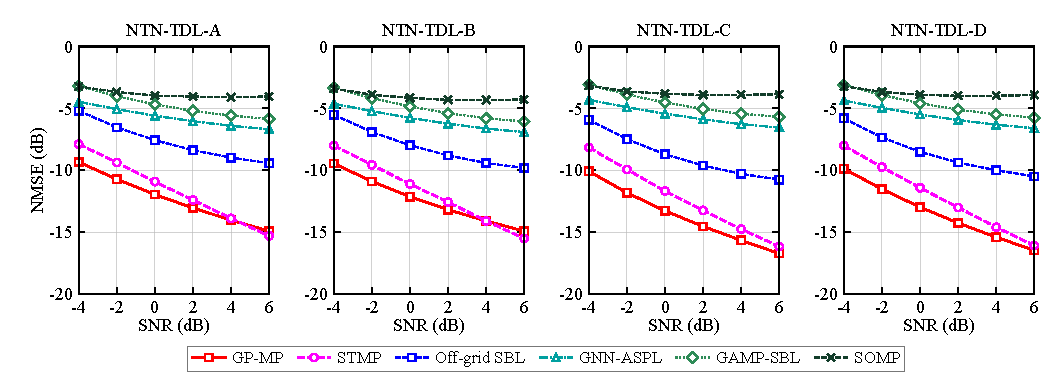
\includegraphics[width=177.8mm]{cross_channel.pdf}
\caption{Channel NMSE for NTN-TDL profiles A, B, C, and D (from left
to right), with $K=40$, $Q=16$, and $p=0.1$.}
\label{fig:cstmp-cross}
\end{figure*}

\subsection{Channel Denoising Performance}
\label{sec:denoising-performance}
We first evaluate the channel denoisers under
$\mathbf R=\mathbf H+\mathbf W$, where
$\vect(\mathbf W)\sim\CN(\mathbf0,v\I)$ and $v$ is known.
The nominal SNR is $-10\log_{10}v$ and takes six values from
$-20$ to $30$~dB. The reference estimators are:
\begin{itemize}[leftmargin=*,topsep=2pt,itemsep=2pt,parsep=0pt]
\item \textbf{Least squares (LS):} The estimate is the noisy observation
$\mathbf R$.
\item \textbf{Gaussian-prior estimate:} The estimate is
$\widehat P_H\mathbf R/(\widehat P_H+v)$, where $\widehat P_H$ is the
training-channel power.
\item \textbf{Genie-aided conditional MMSE:} We compute the analytic
conditional MSE of the remaining Gaussian gains given the true path
geometry, powers, and line-of-sight gain.
\end{itemize}
We also evaluate the four sparse-recovery baselines in this denoising
setting.

Figure~\ref{fig:cstmp-denoising} shows that both learned denoisers
achieve lower NMSE than LS and the Gaussian-prior estimate throughout
the tested SNR range. Their advantage over the sparse-recovery baselines
increases at moderate and high SNR, where these baselines approach error
floors while the NMSE of the learned denoisers continues to decrease.
The GP-MP denoiser yields lower NMSE at low SNR, whereas the STMP
denoiser yields lower NMSE at high SNR.
Both remain above the genie-aided reference.

\subsection{Effect of Density Ratio Estimation}
\label{sec:activity-evidence}
To assess density ratio estimation, we compare the learned activity
update with the Gaussian approximation

\begin{align}
 \ell_k^{\rm G}&=\frac{\norm{\mathbf R_k}_F^2}{v}
 -\frac{\norm{\mathbf R_k-\mathbf E_k}_F^2}{\tau_k^{\rm ext}+v}
 \notag\\
 &\quad-D\log\left(1+\frac{\tau_k^{\rm ext}}{v}\right),
 \label{eq:gaussian-evidence}\\
 p_k&=\sigmoid(\logit\rho+\ell_k^{\rm G}).
 \label{eq:gaussian-activity}
\end{align}

For both STMP and GP-MP, we change only the activity update and keep
the remaining settings fixed. Table~\ref{tab:activity-evidence} reports
the AER over
all runs and the percentage reaching the $600$-iteration limit (Limit).

Table~\ref{tab:activity-evidence} shows that, for both receivers, the
learned activity update yields lower AER than the Gaussian update at
every tested SNR. No run using the learned update reaches the iteration
limit, whereas some runs using the Gaussian update do. The improvement
is larger for GP-MP, although STMP performs better
under the Gaussian update. These results support the effectiveness of
density ratio estimation for activity detection under the learned
channel prior.

\subsection{JADCE Performance}
\label{sec:jadce-performance}
Unless stated otherwise, the default parameters in
Table~\ref{tab:simulation-parameters} are used.

Figure~\ref{fig:cstmp-convergence} compares the NMSE trajectories with
early stopping disabled. The GP-MP curve
stabilizes earlier and at a lower NMSE than STMP. Off-grid SBL also
levels off, but with a larger estimation error. GP-MP therefore achieves
a more accurate channel estimate within fewer iterations than STMP.

Figure~\ref{fig:cstmp-snr} compares channel NMSE and AER over SNRs
from $-4$ to $6$~dB. GP-MP achieves the lowest NMSE throughout this
range, with an approximately $1.5$~dB advantage over STMP at $0$~dB.
Its advantage over STMP decreases as SNR increases, whereas the gap
to the sparse-recovery baselines widens. Off-grid SBL is the most
accurate of the four sparse-recovery baselines, and GP-MP outperforms
all three Off-grid SBL configurations.

The AER also generally decreases with SNR. GP-MP has lower AER than
STMP throughout this SNR range and outperforms the four sparse-recovery
baselines at moderate and high SNR. These results demonstrate improved
JADCE performance with a denoiser that provides channel estimates and
average variance without a separately trained variance model.

With estimated phases, GP-MP-EP incurs an NMSE increase of
$0.28$--$0.60$~dB relative to GP-MP, while its AER remains close to
the known-phase result. This comparison shows that estimating the
phases from pilot observations retains most of the known-phase
receiver's performance over this SNR range.

Figure~\ref{fig:cstmp-pilots} shows channel NMSE as $Q$ increases from
$8$ to $24$. With fixed energy per frame, additional frames provide more
observations and generally reduce NMSE. GP-MP and GP-MP-EP achieve
lower NMSE than all baselines at each frame count. For an NMSE target
of $-12$~dB, both reach the target at $16$ frames, compared with $20$
frames for STMP, corresponding to a $20\%$ reduction in pilot frames.

STMP exhibits severe degradation at low pilot counts: its NMSE is
$34.70$~dB at $Q=8$ and $-4.78$~dB at $Q=12$, compared with
$-8.88$~dB and $-11.61$~dB for GP-MP, respectively. This pronounced
loss indicates that STMP is more sensitive to limited pilot observations.
GP-MP-EP incurs an NMSE increase of $0.30$--$0.41$~dB relative to
GP-MP across these frame counts.

Figure~\ref{fig:cstmp-users} compares NMSE as the number of candidate
devices increases from $K=20$ to $100$. With the activity probability
and pilot-frame count fixed, both the number of candidate channels and
the expected number of active devices increase. The NMSE therefore
increases for all methods. GP-MP
maintains the lowest NMSE, with a growing advantage over STMP as $K$
increases. This demonstrates its effectiveness at higher device loads
with the available pilot and antenna resources.

Figure~\ref{fig:cstmp-activity} shows NMSE for nominal activity
probabilities from $0.05$ to $0.25$. Increasing the activity probability
increases the expected number of active devices, while the numbers of
candidate devices, pilot frames, and receive antennas remain fixed.
The NMSE increases for all methods. GP-MP maintains the lowest NMSE,
with a smaller increase than STMP. Its larger advantage at higher
activity probabilities indicates
better tolerance to increasing activity loads.

\subsection{Comparison Across Channel Profiles}
To examine performance under channel mismatch, we apply the networks
trained on NTN-TDL-D to profiles A, B, and C without retraining.

Figure~\ref{fig:cstmp-cross} shows that GP-MP outperforms the four
sparse-recovery baselines on all four profiles. This indicates that the
learned prior remains effective across these channel profiles. The relative
performance of the two learned receivers depends on the profile and
SNR; STMP is more accurate on profiles A and B at $6$~dB.

\section{Conclusion}
\label{sec:conclusion}

% Included in both manuscript versions on 2026-11-03 at the author's request.
In this paper, we investigated GNSS-independent GFRA for LEO satellite
IoT systems. We proposed a multi-frame AFDM transmission scheme that
accommodates large differential delays and Doppler shifts without
device-side precompensation and derived its input-output relationship.
Additional pilot frames provide more observations without
increasing the number of channel coefficients to be estimated. We learned
a score-based generative prior for AFDM effective channels without imposing
sparse or grid-aligned channel assumptions, and developed a denoiser that
provides channel estimates and average variance without requiring a
separately trained variance model. We incorporated this denoiser into a
message-passing JADCE receiver comprising MFLE and GPJD. The learned
density-ratio estimator in GPJD enables activity detection under the
learned prior without explicit marginal-likelihood evaluation. Simulation
results demonstrated improved activity detection and channel estimation
over the adapted STMP baseline, with fewer pilot frames required for
comparable channel-estimation performance. The receiver also achieved
lower NMSE than the sparse-recovery baselines across the tested NTN-TDL
profiles without retraining.


\ifdefined\FullManuscript
\appendices
\numberwithin{equation}{section}
\section{Receiver Configurations and Evaluation Protocol}
\label{app:evaluation-protocol}

\subsection{Learned Receiver Configurations}
\label{app:receiver-configurations}

The STMP baseline adapts \cite{cai2026} to the AFDM model, replacing
the Gaussian-message-based activity-probability update with learned
density-ratio estimation. It uses a white-noise-trained first-order score network, a
learned second-order score network, and a classifier for density ratio estimation.
GP-MP uses a denoiser trained with white Gaussian noise of covariance
$v\I_D$ and the scalar preconditioning
in Section~\ref{sec:network-settings}, its derivative-based variance
estimate, the corresponding activity classifier, and the input
variance update in Section~\ref{sec:variance-update}.
The two configurations use the same clean training channels and number of
denoiser training epochs.

GP-MP uses the white-noise-trained networks in
Figs.~\ref{fig:cstmp-denoising}--\ref{fig:cstmp-pilots}
and Table~\ref{tab:activity-evidence}; GP-MP-EP in
Figs.~\ref{fig:cstmp-snr} and \ref{fig:cstmp-pilots} uses the same networks.
The GP-MP results in Figs.~\ref{fig:cstmp-users}--\ref{fig:cstmp-cross} use earlier checkpoints
with different training perturbations and await replacement.

The activity-probability comparison in Section~\ref{sec:activity-evidence}
changes only the probability calculation within each receiver.
GP-MP-EP uses the same network weights and message-passing updates
as the corresponding known-phase GP-MP configuration, with phases
estimated once as described in Section~\ref{sec:phase-estimation}.

\subsection{Paired Scenes and Parameter Selection}
\label{app:paired-scenes}

We draw independent Bernoulli activity indicators with nominal probability
$p$ and retain scenes with at least one active device. The receiver uses the
resulting marginal probability $\rho=p/[1-(1-p)^K]$.

The evaluation protocol specifies $1{,}000$ Monte Carlo trials per
operating point. The counts below record the batches currently represented
in the working-draft figures and table; the remaining trials will be
completed before finalizing the corresponding results.

The comparisons in Section~\ref{sec:simulations} use saved, paired physical
scenes, with scene seeds reused across conditions.
The SNR figure uses scenes $0$--$999$ at each point for all
nine configurations. GP-MP-EP uses estimated phases, and the other eight
use known phases.
The pilot comparison reports channel NMSE for all nine configurations
at $Q\in\{8,12,16,20,24\}$, using $500$ paired scenes per point.
The device-count, activity-probability, and cross-profile
comparisons also use scenes $0$--$499$ at each condition.
The channel-denoising comparison uses $2{,}000$ channel samples from
$500$ scenes at each SNR. Both neural denoisers use the same channel
samples and noise realizations. The sparse-recovery baselines use an
identity observation operator and known AWGN variance, retaining their
receiver settings and GNN weights; GAMP-SBL retains its internal
noise-variance update.
The convergence comparison uses $30$ paired
scenes, and the activity-update comparison uses $100$ paired scenes per SNR.
Some evaluation scenes were used during method development and
selection of baseline activity thresholds; the adopted baseline activity decision rules are
reused without refitting. The reported SNR range was narrowed after
interim inspection; the earlier $8$ and $10$~dB results remain archived.
All finite outputs are included in the reported metrics, including those that
reach the iteration limit.

\subsection{Activity Probability Comparison}
\label{app:activity-evidence-protocol}

Table~\ref{tab:activity-evidence} currently uses the first $100$ completed
paired scenes per SNR.
All four variants use the same saved observations, known phases, and
noise variances estimated from the observations, with single-precision
inference and TF32 disabled.
The subset was adopted after interim inspection; the six SNR conditions
reuse the same physical scenes.

The limit rate is the fraction of runs that execute $600$ iterations.

\subsection{Device-Count-Specific Damping}

STMP uses damping factor $0.2$ at $K=20,40$ and $0.1$ at
$K=60,80,100$. The latter was selected after inspecting the original
$500$-scene results with damping factor $0.2$ and a diagnostic test with $12$ inputs at
damping factor $0.1$. All $12$ diagnostic inputs are included in the reported panels.
With the original damping factor, $498$, $479$, and $500$ runs reached the
iteration limit at $K=60,80,100$, respectively; those outputs remain
archived. Under the adopted settings, all $500$ runs satisfy the stopping criterion at
$K=20,40,60$, while $3$ and $14$ reach the limit at $K=80$ and $100$.

For GP-MP, the damping factor was reduced from $0.4$ to $0.2$ for all
$K=100$ scenes after preliminary inspection. At $K=80$, only scene~372
was rerun with damping factor $0.2$ after its original run reached the iteration
limit; this selected replacement is used in the reported panel. Other
$K=80$ scenes retain damping factor $0.4$. Both receivers retain the same
$60$--$600$ iteration limits and stopping criteria.
These damping factors were selected retrospectively.

\subsection{Convergence and Channel-Profile Evaluation}

Figure~\ref{fig:cstmp-convergence} uses the first $30$ paired scenes
at $0$~dB. For this experiment, GP-MP uses the AWGN-trained denoiser
and its matched activity classifier. GP-MP, STMP, and the baseline Off-grid SBL configuration
each execute $300$ iterations with early stopping disabled; the figure
shows the first $150$ iterations. At each iteration, NMSE is computed
from the total error energy divided by the total active-channel energy
over these scenes, followed by conversion to dB.

In the $1{,}000$-scene-per-SNR experiment displayed in
Fig.~\ref{fig:cstmp-snr}, STMP and GP-MP reach the iteration limit
in one and three runs, respectively, all at $-4$~dB. GP-MP-EP reaches
the limit in two runs, one at $-4$~dB and one at $-2$~dB. The remaining
outputs of these three configurations satisfy the stopping criterion.

The activity-probability and cross-profile sweeps retain damping factors $0.2$
for STMP and $0.4$ for GP-MP. All $2{,}500$ proposed-receiver
runs in the activity-probability experiment meet the stopping criterion. STMP reaches the limit in one
scene at each of $p=0.20$ and $0.25$.
The activity sampling and receiver prior are as defined in
Appendix~\ref{app:paired-scenes}; the horizontal axis denotes
the nominal probability $p$.

For the cross-profile comparison, all $12{,}000$ outputs of each learned
receiver satisfy the receiver stopping criterion.
The experiment varies the tabulated power delay profiles and
fading distributions at fixed geometry, pilots, and receiver settings,
without retraining or changing the stopping rules. Path gains remain fixed within each block, so the comparison concerns
the evaluated delay and fading profiles.

\subsection{Additional Implementation Settings}
\label{app:implementation-settings}

Each training or validation scene supplies four clean channel samples
before multiplication by $\alpha_k$. Denoiser model selection uses fixed
validation-noise realizations. The classifier is randomly initialized
and trained with the denoiser fixed.

For phase estimation, each L-BFGS-B refinement is restricted to a
differentiable interval of the waveform. Coordinate refinement starts
from zero powers and uses two sweeps in descending order of initial
pilot-correlation scores, with the current parameters retained among
the candidates.

The normalization constant is $s=0.2647966453$.
The tolerances for changes in activity probabilities and site parameters,
and for deviations from the moving average of activity probabilities
are $10^{-3}$, $0.1$, and $10^{-3}$, respectively, with
$\zeta_{\rm hist}=0.2$, $L_s=5$, and $L_d=10$.

The stopping rule monitors relative changes in $\widehat{\mathbf X}$ and $v$,
the maximum change in activity probability $\max_k|p_k^{(i)}-p_k^{(i-1)}|$, and
$d_{\rm var}^{(i)}=|v_{\rm tar}^{(i)}-v^{(i)}|/
\max\{v_{\rm tar}^{(i)},v^{(i)}\}$.
It also requires accepted site updates with stable precision
$(\tau_k^{\rm ext})^{-1}$ and natural parameter $\mathbf E_k/\tau_k^{\rm ext}$, together with a small difference from the previous exponential moving average, $\max_k|p_k^{(i)}-w_k^{(i-1)}|$.
After this comparison, update
$w_k^{(i)}=(1-\zeta_{\rm hist})w_k^{(i-1)}+\zeta_{\rm hist} p_k^{(i)}$, starting from
$w_k^{(0)}=\rho$.
After $I_{\min}$ iterations, all these conditions must hold for $L_s$
consecutive iterations and hard activity decisions must remain unchanged
for $L_d$ iterations; otherwise, return the last iterate at $I_{\max}$.


\fi

\bibliographystyle{IEEEtran}
\bibliography{references}
\end{document}

